\documentclass[11pt,a4paper]{article}

% ---------------------------------------------------------------- packages
\usepackage[margin=2.2cm]{geometry}
\usepackage[T1]{fontenc}
\usepackage{lmodern}
\usepackage{microtype}
\usepackage{amsmath,amssymb}
\usepackage{graphicx}
\usepackage{booktabs}
\usepackage{tabularx}
\usepackage{array}
\usepackage{float}
\usepackage{caption}
\usepackage{subcaption}
\usepackage{enumitem}
\usepackage[table]{xcolor}
\usepackage{hyperref}

\graphicspath{{./}}  % all figures live next to this file (assets/)
\definecolor{linkblue}{HTML}{1C5CAB}
\hypersetup{colorlinks=true, linkcolor=linkblue, urlcolor=linkblue, citecolor=linkblue}
\captionsetup{font=small, labelfont=bf}
\setlist{itemsep=2pt, topsep=4pt}
\newcolumntype{Y}{>{\raggedright\arraybackslash}X}
\newcommand{\githuburl}{https://github.com/your-username/deepfake-ml-hackathon}  % TODO: replace with the real repository

\title{\textbf{Deepfake Detection with a LoRA-Tuned Multi-Backbone Ensemble}\\[4pt]
\large IIIT Bangalore Deepfake ML Hackathon --- Technical Report}
\author{Team name / members (TODO)\\[2pt]
\small Code: \href{\githuburl}{\texttt{\githuburl}}}
\date{November 2026}

\begin{document}
\maketitle

\begin{abstract}
\noindent We classify $224\times224$ face crops as real or deepfake. The final model averages three ImageNet-pretrained backbones of different families --- EfficientNet-B4, ConvNeXt-Tiny and Swin-Tiny --- each fine-tuned with low-rank adapters (LoRA, 2--5\% of the weights) and trained with binary cross-entropy plus a two-view consistency loss and a supervised contrastive loss. The ensemble reaches \textbf{0.909 validation AUC} (F1 0.856, accuracy 0.859) against labels in which we find $\approx$8\% to be flipped, which caps the attainable AUC near 0.92. A Streamlit demo with per-model Grad-CAM explains each prediction.
\end{abstract}

% =====================================================================
\section{Problem Statement and Exploratory Data Analysis}

\subsection{Problem}
Given a face image, predict the probability that it is a deepfake (label 1) rather than real (label 0). Submissions are scored on AUC-ROC on a hidden test set (50 pts), inference time on an NVIDIA T4 (20 pts), AUC stability on undisclosed degraded variants of the test set (20 pts) and documentation (10 pts). Only the provided data and ImageNet-pretrained models may be used, and test images may not be used for training in any way.

\subsection{Data}
\begin{table}[H]
\centering\small
\begin{tabular}{@{}lrl@{}}
\toprule
 & Count & Notes \\
\midrule
Training images & 7{,}000 & 3{,}478 real, 3{,}522 fake (\texttt{ground\_truth.csv}) \\
Test images & 3{,}000 & unlabelled \\
Format & --- & $224\times224$ RGB JPEG, face-centred, identical JPEG quantisation tables \\
Duplicates & 0 & none within train or between train and test (MD5) \\
\bottomrule
\end{tabular}
\caption{Dataset summary.}
\end{table}

\begin{figure}[H]
\centering
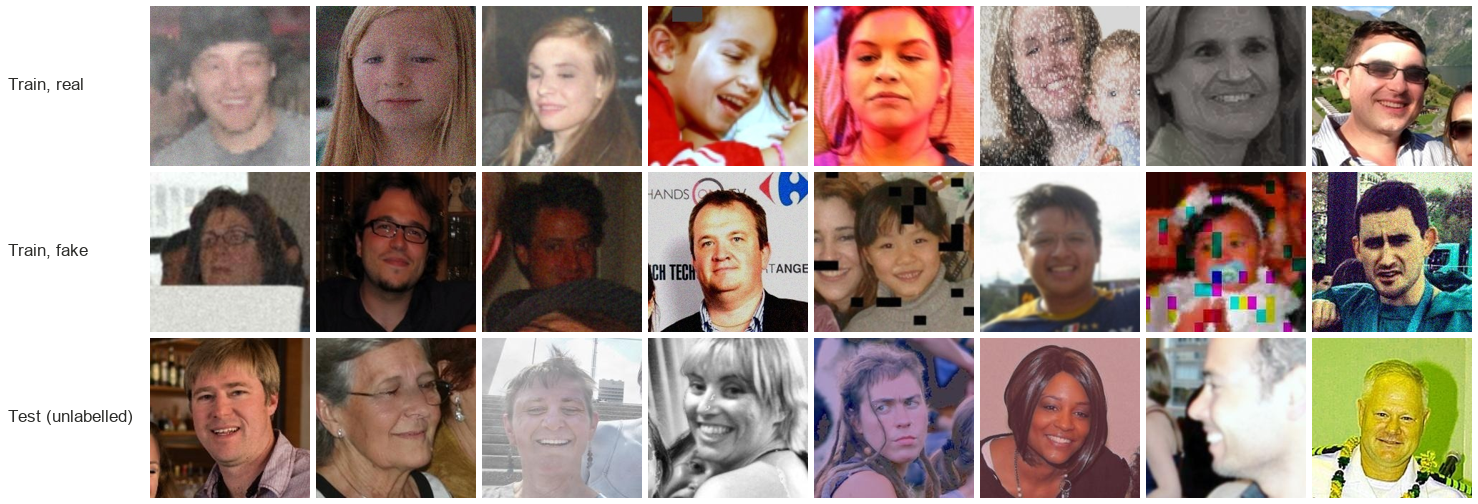
\includegraphics[width=\linewidth]{eda_samples.png}
\caption{Random samples. Real and fake images look alike; many carry heavy synthetic degradations (noise, blur, occlusion boxes, colour shifts, pixelation, block dropout).}
\label{fig:samples}
\end{figure}

\subsection{Corruptions}
About half of all images are deliberately degraded (Table~\ref{tab:corr}, measured with simple pixel-statistic detectors). The same families occur in train and test, in slightly different proportions.

\begin{table}[H]
\centering\small
\begin{tabular}{@{}lrrr@{}}
\toprule
Corruption & Train real & Train fake & Test \\
\midrule
Heavy Gaussian noise & 22.3\% & 22.5\% & 12.1\% \\
Impulse / snow noise & 20.3\% & 18.3\% & 15.3\% \\
Strong blur & 11.9\% & 14.4\% & 7.7\% \\
Flat patches (occlusion boxes, blown highlights) & 11.6\% & 15.9\% & 15.3\% \\
Greyscale & 2.3\% & 2.9\% & 3.9\% \\
Pixelation / block dropout & 1.1\% & 1.7\% & 0.8\% \\
\midrule
Any of the above & 53.3\% & 56.8\% & 46.6\% \\
\bottomrule
\end{tabular}
\caption{Share of images with each corruption.}
\label{tab:corr}
\end{table}

\subsection{Key findings}
\begin{itemize}
\item \textbf{No shortcut signal.} File size, brightness, contrast, sharpness, noise level and JPEG tables separate the classes at only 0.46--0.58 AUC; the signal must be learned from image content.
\item \textbf{Mild train/test shift.} A linear model on ImageNet features distinguishes train from test images at 0.70 AUC, driven mostly by the corruption mix (test images are slightly cleaner).
\item \textbf{Label noise ($\approx$8\%).} \texttt{ground\_truth.csv} is ordered real-first / fake-second with a sharp boundary at row 3{,}500, yet 560 labels (8.0\%) disagree with that order (291 + 269). A linear probe trained only on the official labels scores those images at 0.23 AUC against their official labels and 0.77 against the ordering --- they behave like flipped labels. The organisers' README states the noise is intentional. With a symmetric noise rate $r$, a perfect model scores at most $1-r \approx 0.92$ AUC against these labels.
\item \textbf{Repeated source photos.} Some photographs appear several times under different corruptions, so a random validation split is slightly optimistic.
\end{itemize}

% =====================================================================
\section{Solution Architecture}

\begin{figure}[H]
\centering
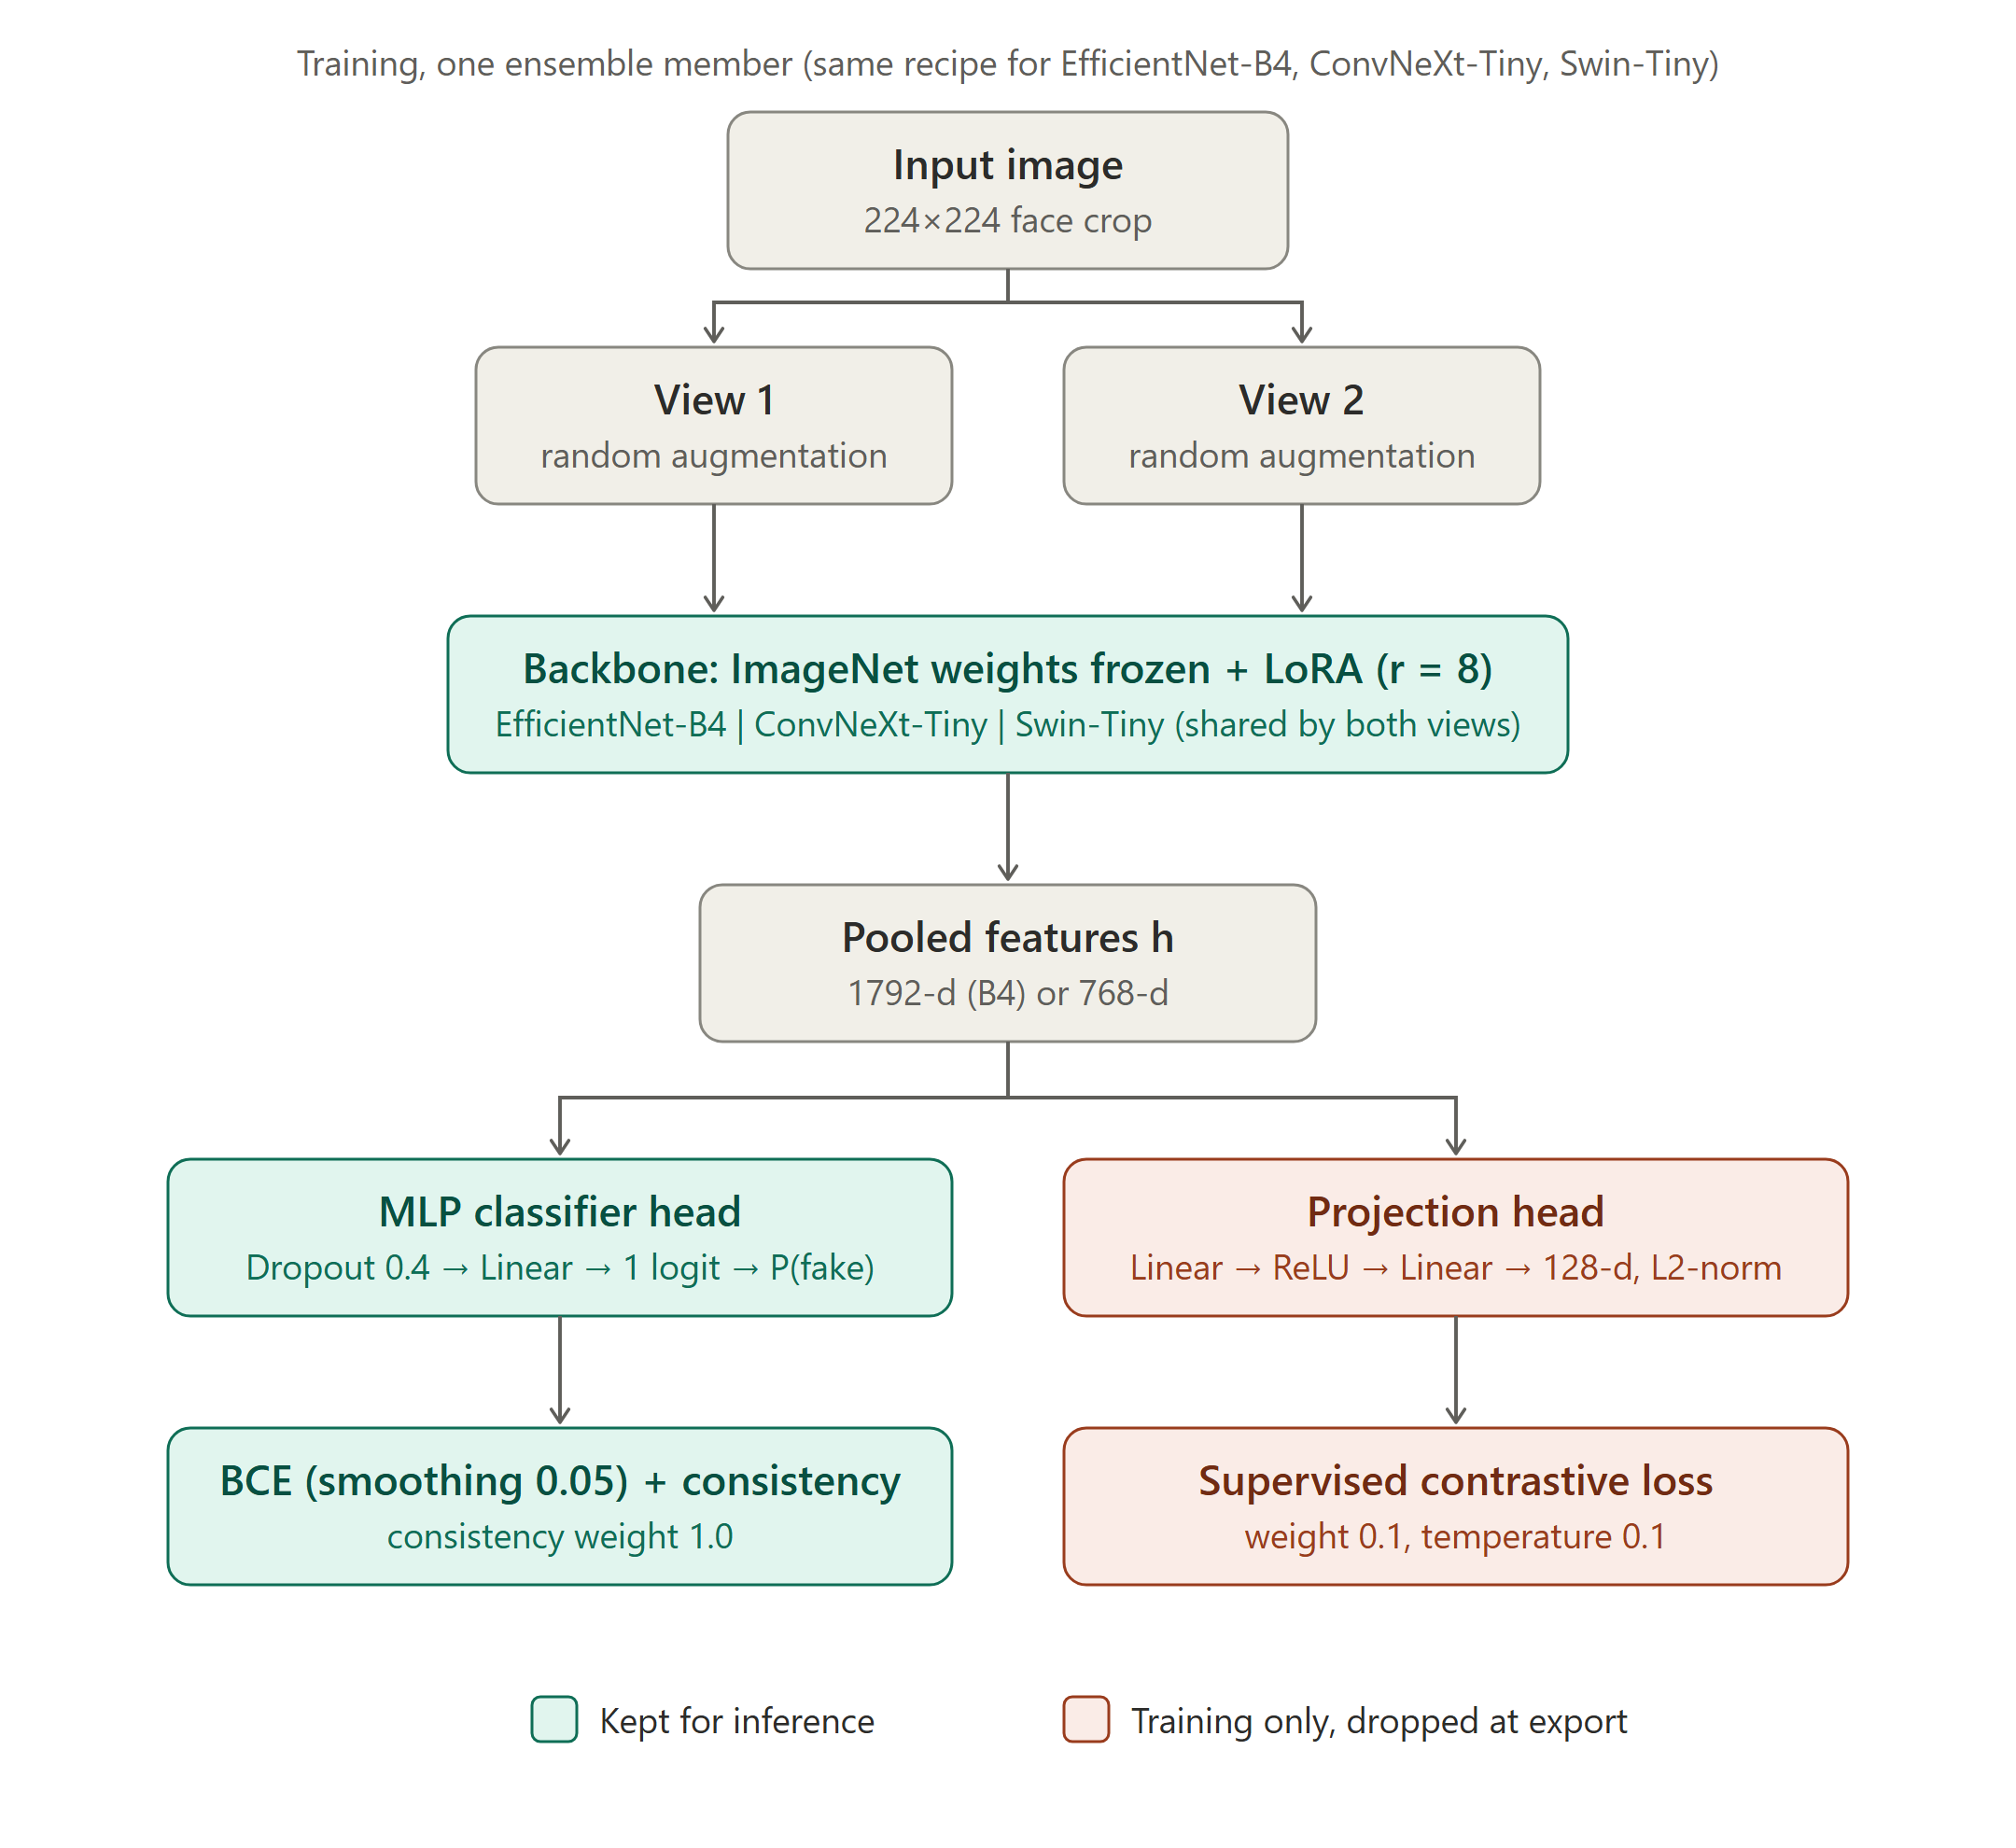
\includegraphics[width=0.78\linewidth]{architecture_training.png}
\caption{Training of one ensemble member (identical recipe for all three backbones). Both augmented views share the backbone; teal parts are kept for inference, the coral projection branch is used only for the contrastive loss.}
\label{fig:arch-train}
\end{figure}

\begin{figure}[H]
\centering
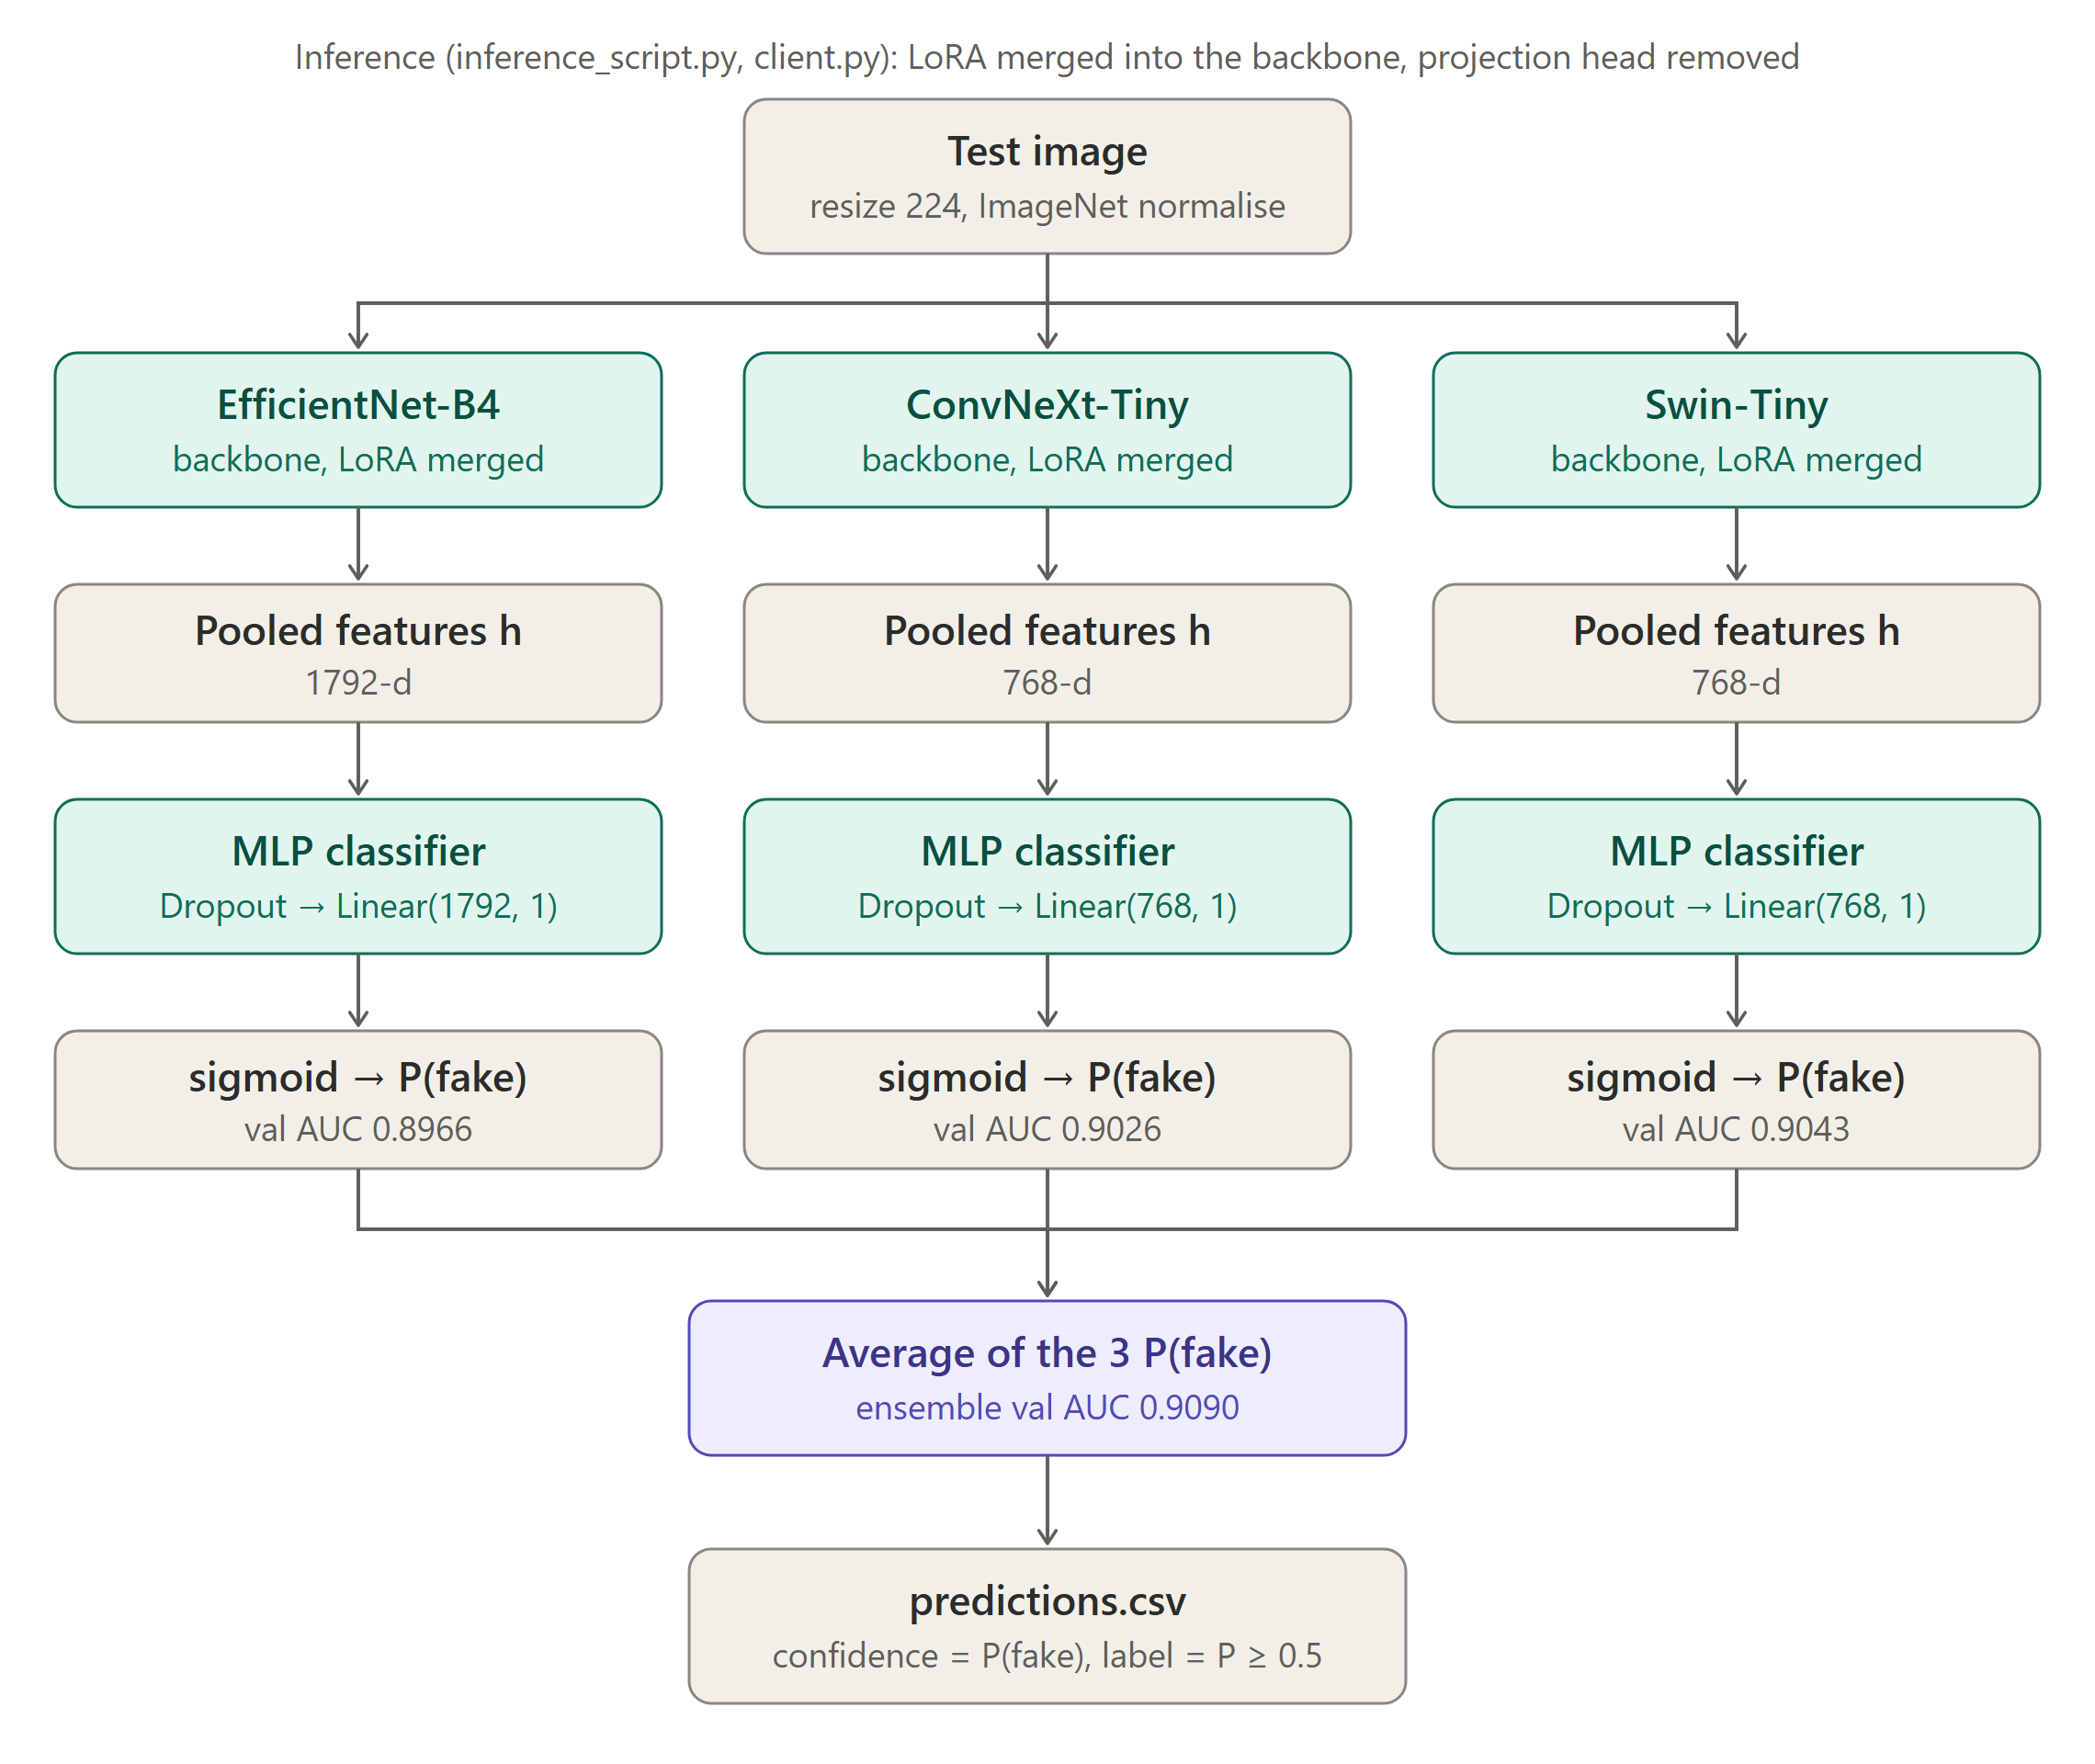
\includegraphics[width=0.82\linewidth]{architecture_inference.png}
\caption{Inference: LoRA is merged into each backbone, the projection head is removed, and every model passes its pooled features through its MLP classifier; the three probabilities are averaged.}
\label{fig:arch-infer}
\end{figure}

\subsection{Backbones}
All three use torchvision ImageNet-1k weights; their ImageNet classifier is replaced by \texttt{Dropout(0.4)} $\rightarrow$ \texttt{Linear(features, 1)}.
\begin{itemize}
\item \textbf{EfficientNet-B4} --- compound-scaled CNN of depthwise-separable MBConv blocks with squeeze-and-excitation (1792-d features).
\item \textbf{ConvNeXt-Tiny} --- modernised ResNet-style CNN with large $7\times7$ depthwise kernels and LayerNorm (768-d).
\item \textbf{Swin-Tiny} --- hierarchical vision transformer with shifted-window self-attention, a different inductive bias from the two CNNs (768-d).
\end{itemize}

\subsection{Fine-tuning strategy}
The pretrained weights stay frozen; we train only rank-8 LoRA adapters ($\alpha=16$, dropout 0.1) --- on EfficientNet's $1\times1$ convolutions and on every linear layer of ConvNeXt and Swin --- plus the new classifier head (Table~\ref{tab:params}). Training so few parameters limits memorisation of the noisy labels. Each image is augmented twice per step, with degradations that mimic the test set; at export LoRA is merged into the weights and the projection head dropped, so inference runs plain backbones at full speed.

\begin{table}[H]
\centering\small
\begin{tabular}{@{}lllr@{}}
\toprule
Backbone & LoRA targets & Frozen params & Trainable (kept) \\
\midrule
EfficientNet-B4 & all $1\times1$ convolutions & 17.5M & 1.01M (5.4\%) \\
ConvNeXt-Tiny & all \texttt{nn.Linear} (pointwise MLPs) & 27.8M & 0.53M (1.9\%) \\
Swin-Tiny & all \texttt{nn.Linear} (attention + MLP) & 27.5M & 0.60M (2.1\%) \\
\bottomrule
\end{tabular}
\caption{Parameter budget per model. The training-only projection head (\texttt{Linear}$\rightarrow$\texttt{ReLU}$\rightarrow$\texttt{Linear}, 128-d) is not counted.}
\label{tab:params}
\end{table}

\paragraph{Augmentation.} Resize to 224, horizontal flip, colour jitter ($p=0.5$), Gaussian blur ($p=0.2$), and test-like degradations: pixelation (downscale to 32--64\,px, nearest upscale; $p=0.15$), greyscale ($p=0.1$), posterise to 2 bits ($p=0.1$), solarise ($p=0.05$), random erasing with random-colour blocks ($p=0.25$). Validation and test use resize + ImageNet normalisation only.

\subsection{Loss}
For $B$ images ($2B$ views) with logit $z$, $p=\sigma(z)$, smoothed target $t = y(1-\varepsilon)+\varepsilon/2$ ($\varepsilon=0.05$) and L2-normalised projection embedding $e$:
\begin{equation}
\mathcal{L} =
\underbrace{-\frac{1}{2B}\sum_{i}\Big[t_i\log p_i+(1-t_i)\log(1-p_i)\Big]}_{\text{BCE}}
\;+\;1.0\,\underbrace{\frac{1}{B}\sum_{j}\big(p_j^{(1)}-p_j^{(2)}\big)^2}_{\text{two-view consistency}}
\;+\;0.1\,\underbrace{\Bigg(-\frac{1}{2B}\sum_{i}\frac{1}{|P(i)|}\sum_{q\in P(i)}\log\frac{\exp(e_i\!\cdot e_q/\tau)}{\sum_{a\neq i}\exp(e_i\!\cdot e_a/\tau)}\Bigg)}_{\text{supervised contrastive},\ \tau=0.1}
\end{equation}
\textbf{Intuition.} BCE learns real vs.\ fake; the consistency term makes both augmented views of an image receive the same score, so blur, noise or pixelation must not change the verdict; the contrastive term ($P(i)$ = other inputs with the same label) pulls same-class embeddings together, shaping the shared backbone through the LoRA adapters.

\subsection{Training configuration}
\begin{table}[H]
\centering\small
\begin{tabular}{@{}ll@{}}
\toprule
Setting & Value \\
\midrule
Split & 80/20 random split (seed 42), identical for all models; 5{,}600 train / 1{,}400 validation \\
Optimiser & AdamW, learning rate $3\times10^{-4}$, weight decay $10^{-4}$ \\
Schedule & cosine annealing over 20 epochs \\
Batch & 32 images (64 augmented views), mixed precision (AMP) \\
Model selection & epoch with the best validation AUC (official labels) \\
Hardware & Kaggle, NVIDIA T4 \\
Ensemble & mean of the three models' P(fake); label = P(fake) $\geq 0.5$ \\
\bottomrule
\end{tabular}
\caption{Training setup.}
\end{table}

% =====================================================================
\section{Results}

All validation numbers are on the 1{,}400 held-out images with the official (noisy) labels and threshold 0.5.

\subsection{Single models and ensembles}
\begin{table}[H]
\centering\small
\begin{tabular}{@{}lrrrr@{}}
\toprule
Model & Best epoch & Val AUC & Val F1 & Val accuracy \\
\midrule
EfficientNet-B4 & 18 & 0.8966 & 0.8346 & 0.8386 \\
ConvNeXt-Tiny & 6 & 0.9026 & 0.8418 & 0.8464 \\
Swin-Tiny & 11 & 0.9043 & 0.8573 & 0.8571 \\
\midrule
\rowcolor{gray!12}\textbf{B4 + ConvNeXt + Swin (submitted)} & --- & \textbf{0.9090} & 0.8559 & 0.8586 \\
ConvNeXt + Swin & --- & 0.9081 & 0.8598 & 0.8621 \\
B4 + Swin & --- & 0.9066 & 0.8604 & 0.8621 \\
B4 + ConvNeXt & --- & 0.9060 & 0.8489 & 0.8536 \\
\bottomrule
\end{tabular}
\caption{Validation metrics. Ensembles average probabilities.}
\label{tab:results}
\end{table}

The models are related but not redundant: their validation predictions correlate at 0.914 (B4--ConvNeXt), 0.911 (B4--Swin) and 0.931 (ConvNeXt--Swin), so averaging adds +0.005 AUC over the best single model.

\begin{figure}[H]
\centering
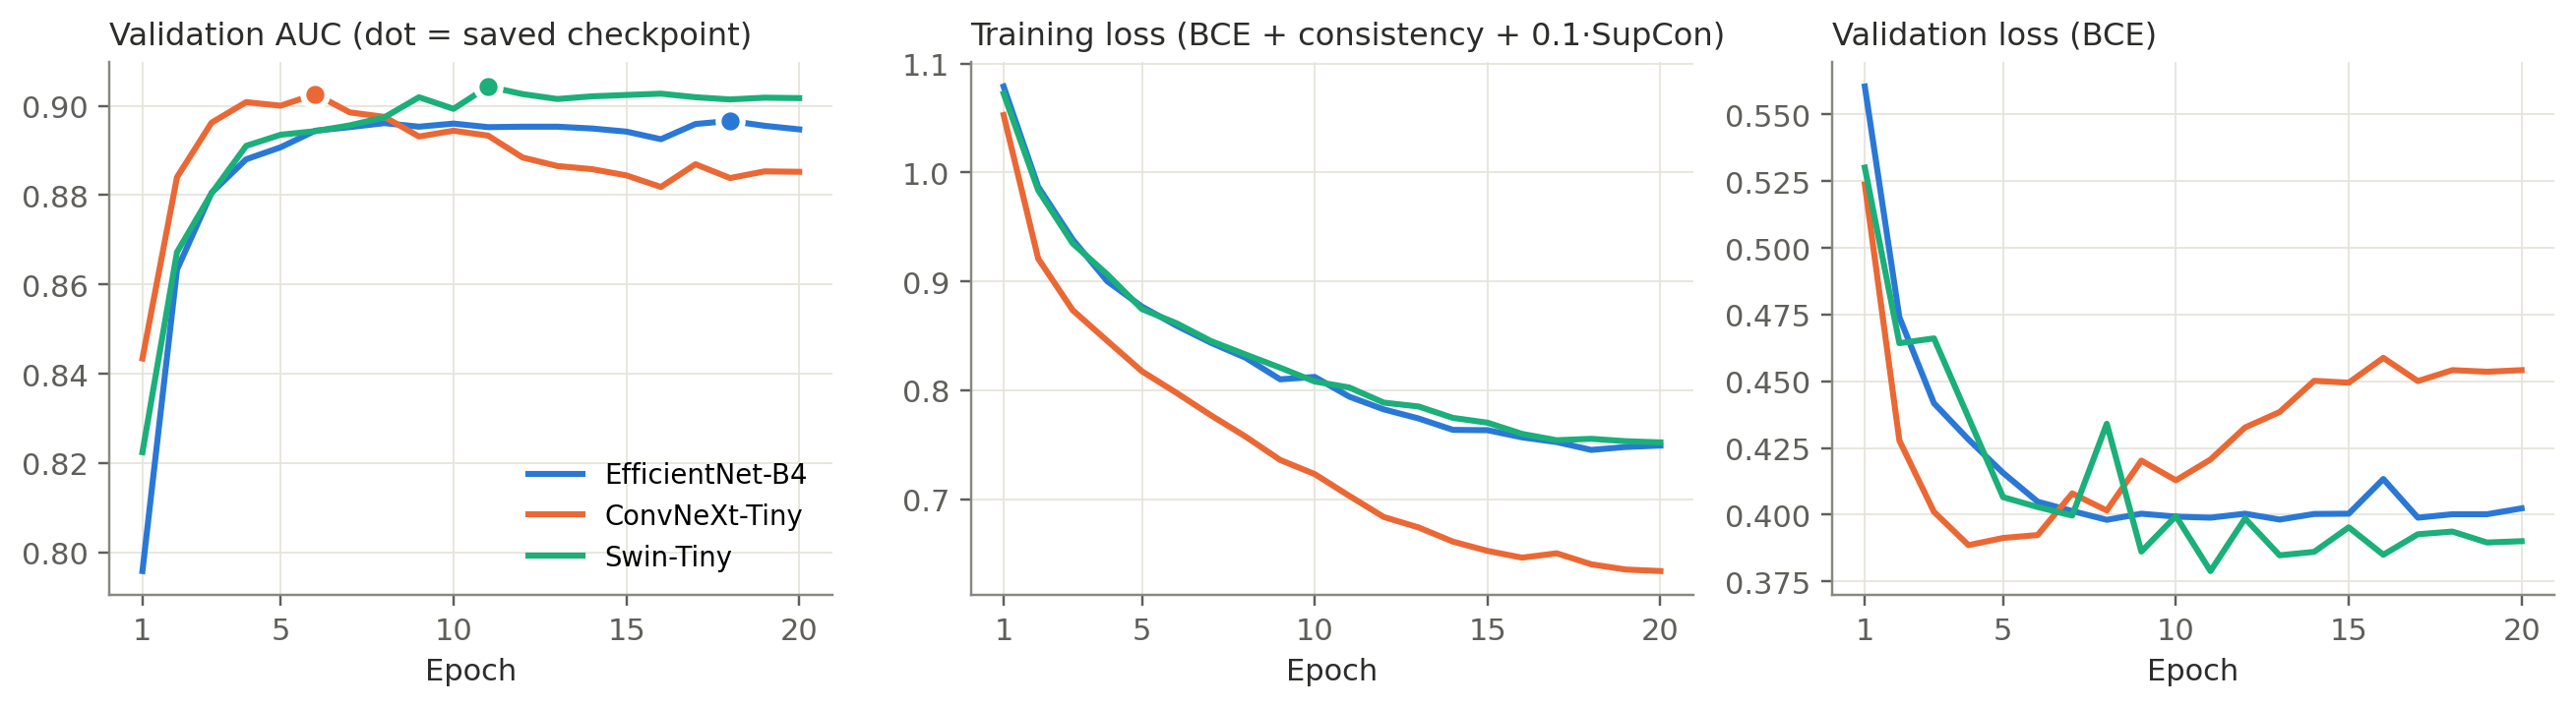
\includegraphics[width=\linewidth]{training_curves.png}
\caption{Training curves from the Kaggle runs. ConvNeXt peaks early and then overfits (validation loss rises from epoch 6); checkpoint selection on validation AUC keeps the epoch-6 weights. EfficientNet and Swin plateau.}
\label{fig:curves}
\end{figure}

\begin{figure}[H]
\centering
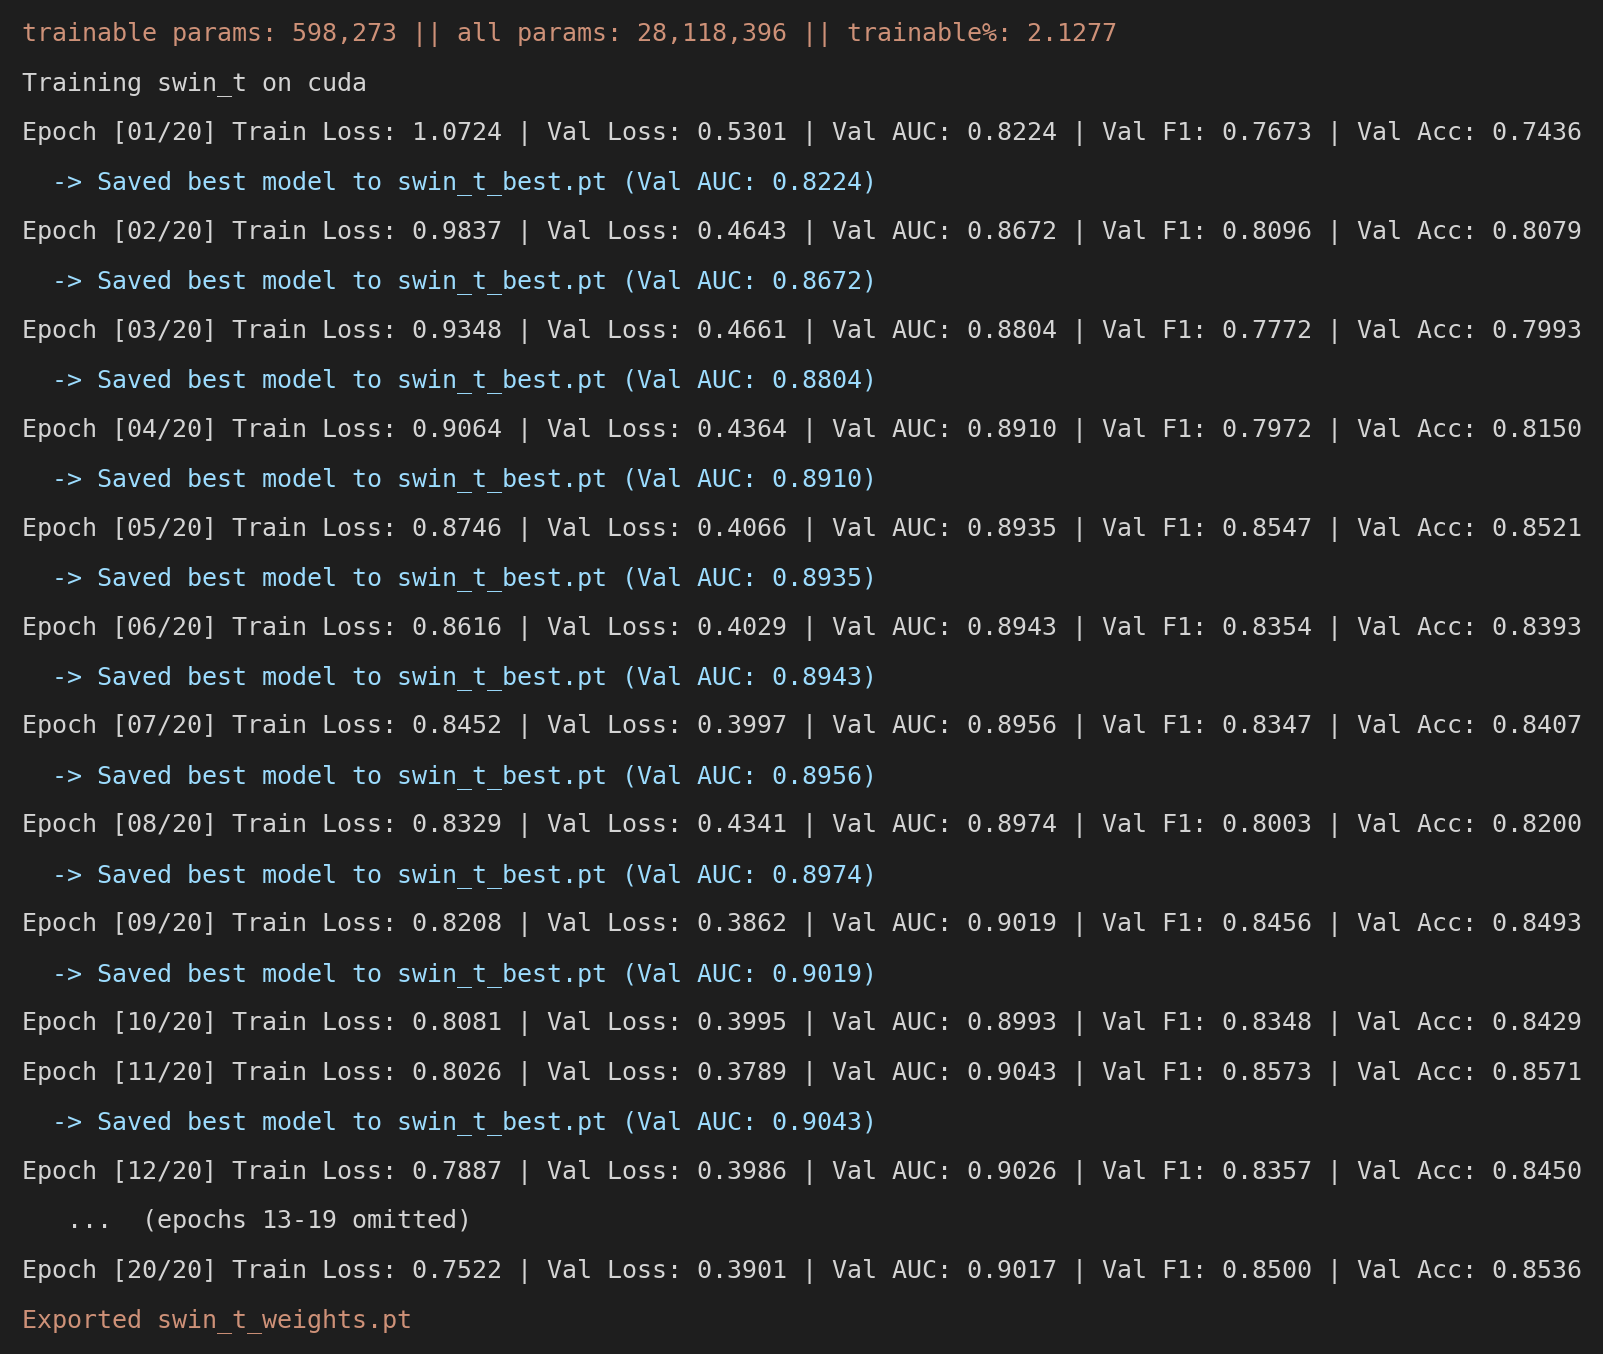
\includegraphics[width=0.9\linewidth]{training_log_swin.png}
\caption{Excerpt of the notebook training log for Swin-Tiny (best checkpoint at epoch 11, AUC 0.9043).}
\label{fig:log}
\end{figure}

\begin{figure}[H]
\centering
\begin{subfigure}[t]{0.56\linewidth}\centering
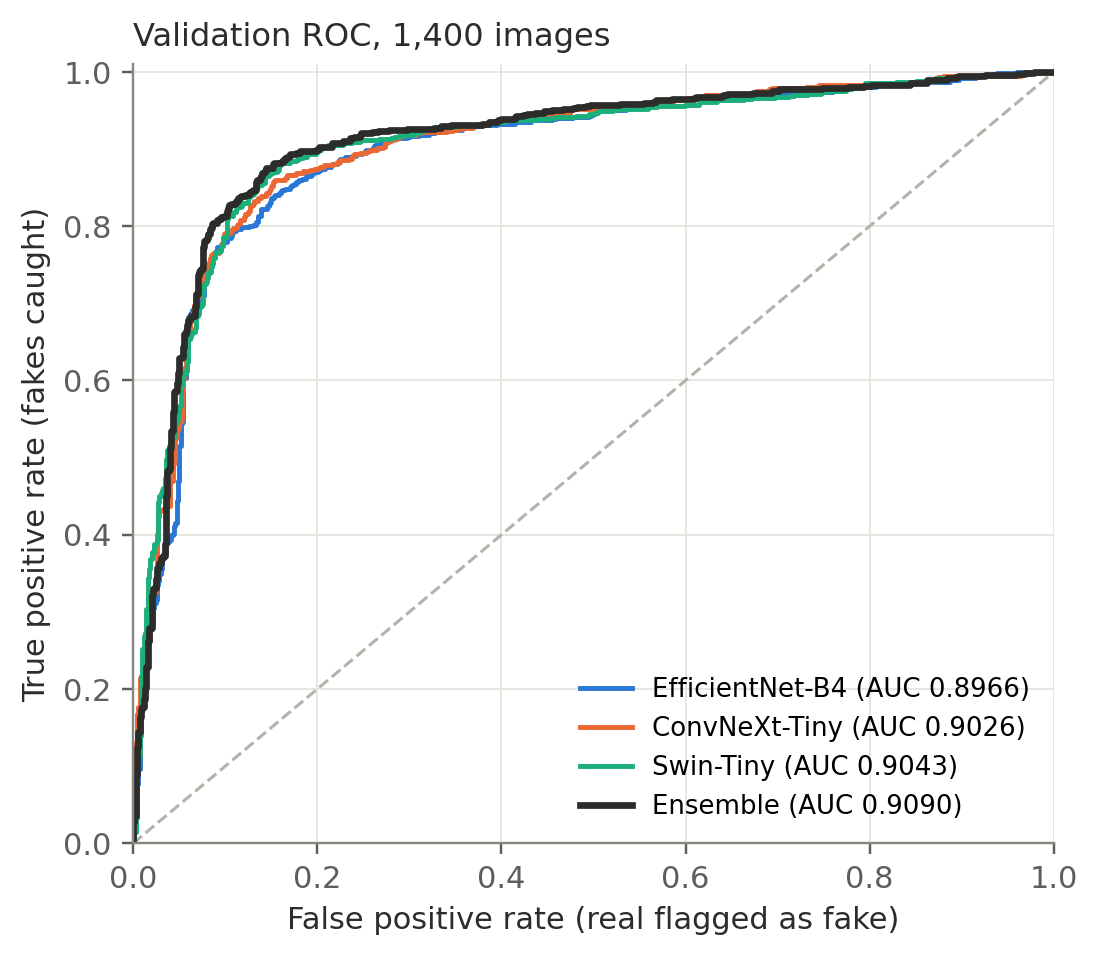
\includegraphics[width=\linewidth]{val_roc.png}
\caption{ROC curves on the validation set.}
\end{subfigure}\hfill
\begin{subfigure}[t]{0.40\linewidth}\centering
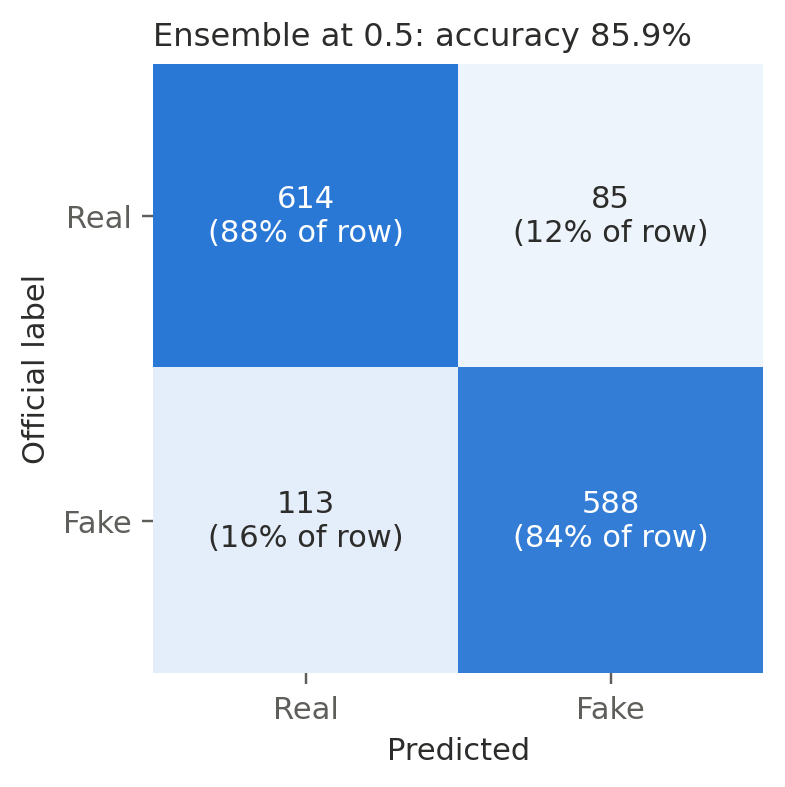
\includegraphics[width=\linewidth]{val_confusion.png}
\caption{Ensemble confusion matrix at 0.5.}
\end{subfigure}
\caption{Validation ROC and confusion matrix, recomputed from the submitted checkpoints (AUCs match the training logs exactly). At threshold 0.5 the ensemble catches 84\% of fakes and flags 12\% of real images; part of these errors are the flipped labels.}
\label{fig:roc}
\end{figure}

\begin{figure}[H]
\centering
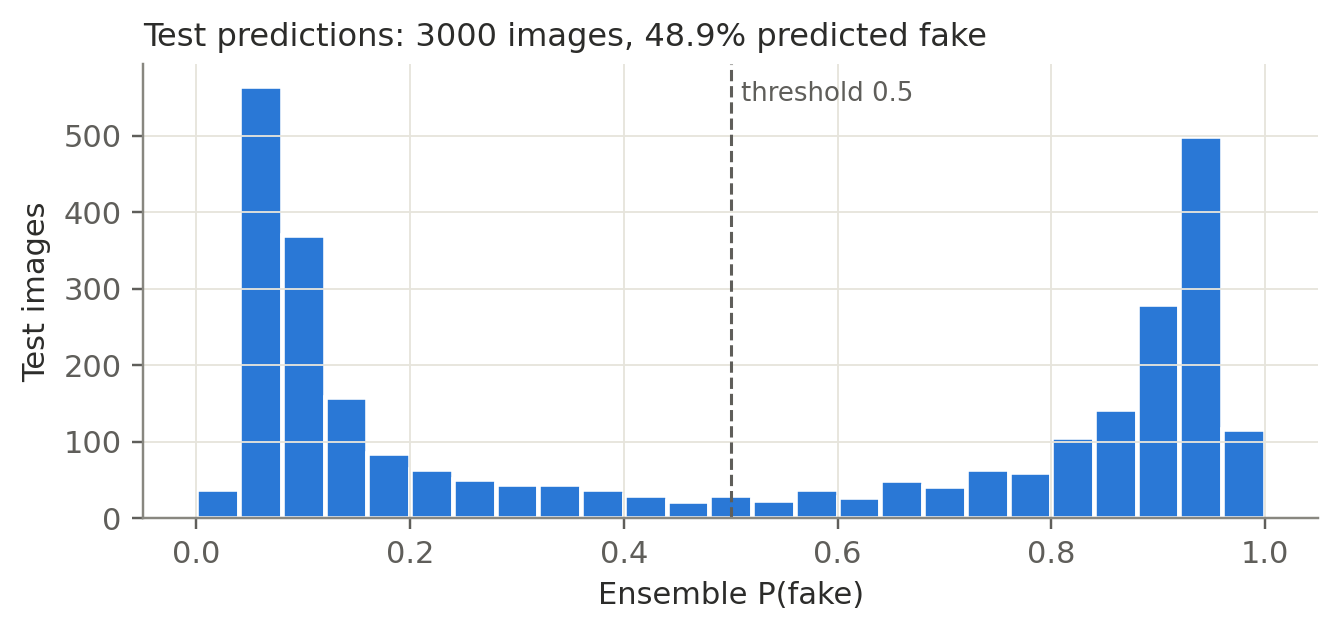
\includegraphics[width=0.62\linewidth]{test_confidence_hist.png}
\caption{Ensemble confidence on the 3{,}000 test images: clearly bimodal, 48.9\% predicted fake (training set: 50.3\% fake).}
\label{fig:testhist}
\end{figure}

\subsection{Development history and ablation}
\begin{table}[H]
\centering\small
\begin{tabularx}{\linewidth}{@{}Yr@{}}
\toprule
Configuration & Val AUC \\
\midrule
EfficientNet-B4, frozen backbone + linear head$^{\dagger}$ & 0.702 \\
EfficientNet-B4, LoRA, light augmentation, BCE only$^{\dagger}$ & 0.886 \\
EfficientNet-B4, LoRA + test-like degradations + consistency + SupCon & 0.895 \\
Ensemble of three backbones (v1, \textbf{submitted}) & \textbf{0.909} \\
\midrule
Heavier head: MLP neck, multi-scale tokens, attention pooling, patch head, trainable norms (+1.1M params on B4), 3-model ensemble & 0.907 \\
\quad same, horizontal-flip test-time averaging & 0.908 \\
\bottomrule
\end{tabularx}
\caption{What moved the score. LoRA fine-tuning was the largest gain; robustness-oriented augmentation and the auxiliary losses added a little; architectural diversity added +0.005 via the ensemble. The heavier head gave no improvement, so the simpler v1 was kept. $^{\dagger}$Validated on augmented images (earlier protocol), so not strictly comparable.}
\label{tab:ablation}
\end{table}

\subsection{Reproducibility and efficiency}
\begin{itemize}
\item \texttt{inference\_script.py} reproduces the submitted \texttt{predictions.csv} on all 3{,}000 images with \textbf{0 label differences} (largest confidence difference 0.002, FP32 on CPU vs.\ FP16 on GPU).
\item Inference is batched (64 images) with FP16 autocast and 4 data-loading workers; the three backbones total about 10.5 GFLOPs per image. On CPU the full test set takes 9--14 minutes; T4 timing: \textbf{TODO}.
\item Code, commands and the training notebook (with full logs): \href{\githuburl}{\texttt{\githuburl}}.
\end{itemize}

% =====================================================================
\section{Explainability and Live Demo}

A Streamlit app (\texttt{client.py}) loads the same models and preprocessing as the inference script. For an uploaded image it shows the ensemble verdict, each model's P(fake) against the decision threshold, and Grad-CAM maps for every model plus their average.

\begin{figure}[H]
\centering
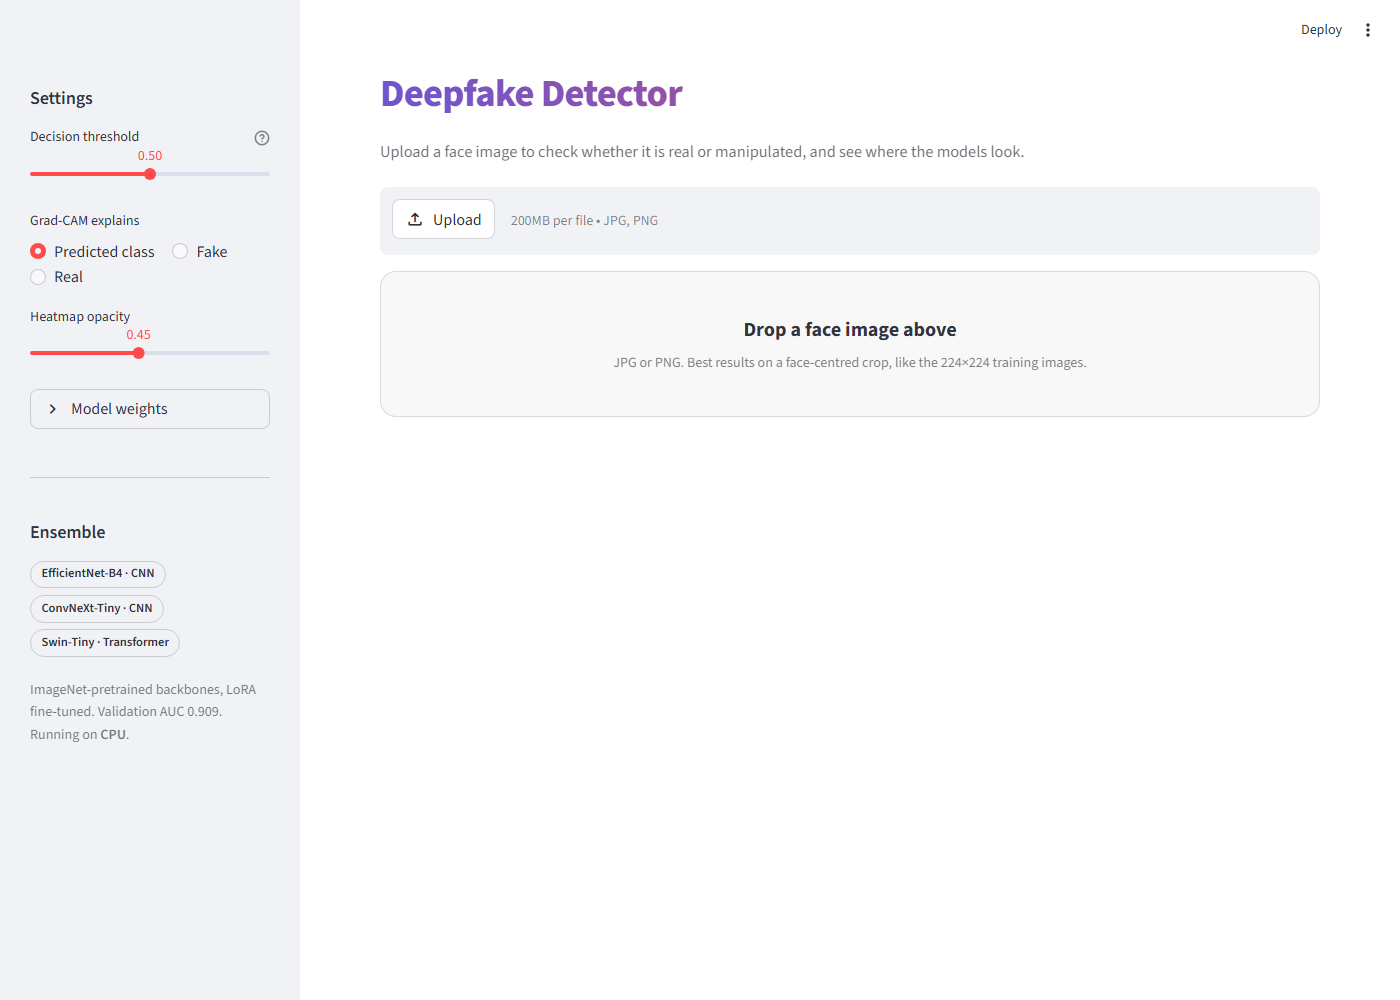
\includegraphics[width=0.85\linewidth]{streamlit_home.png}
\caption{Home screen. Sidebar: decision threshold, Grad-CAM target, heatmap opacity, weights path, ensemble members.}
\end{figure}

\begin{figure}[H]
\centering
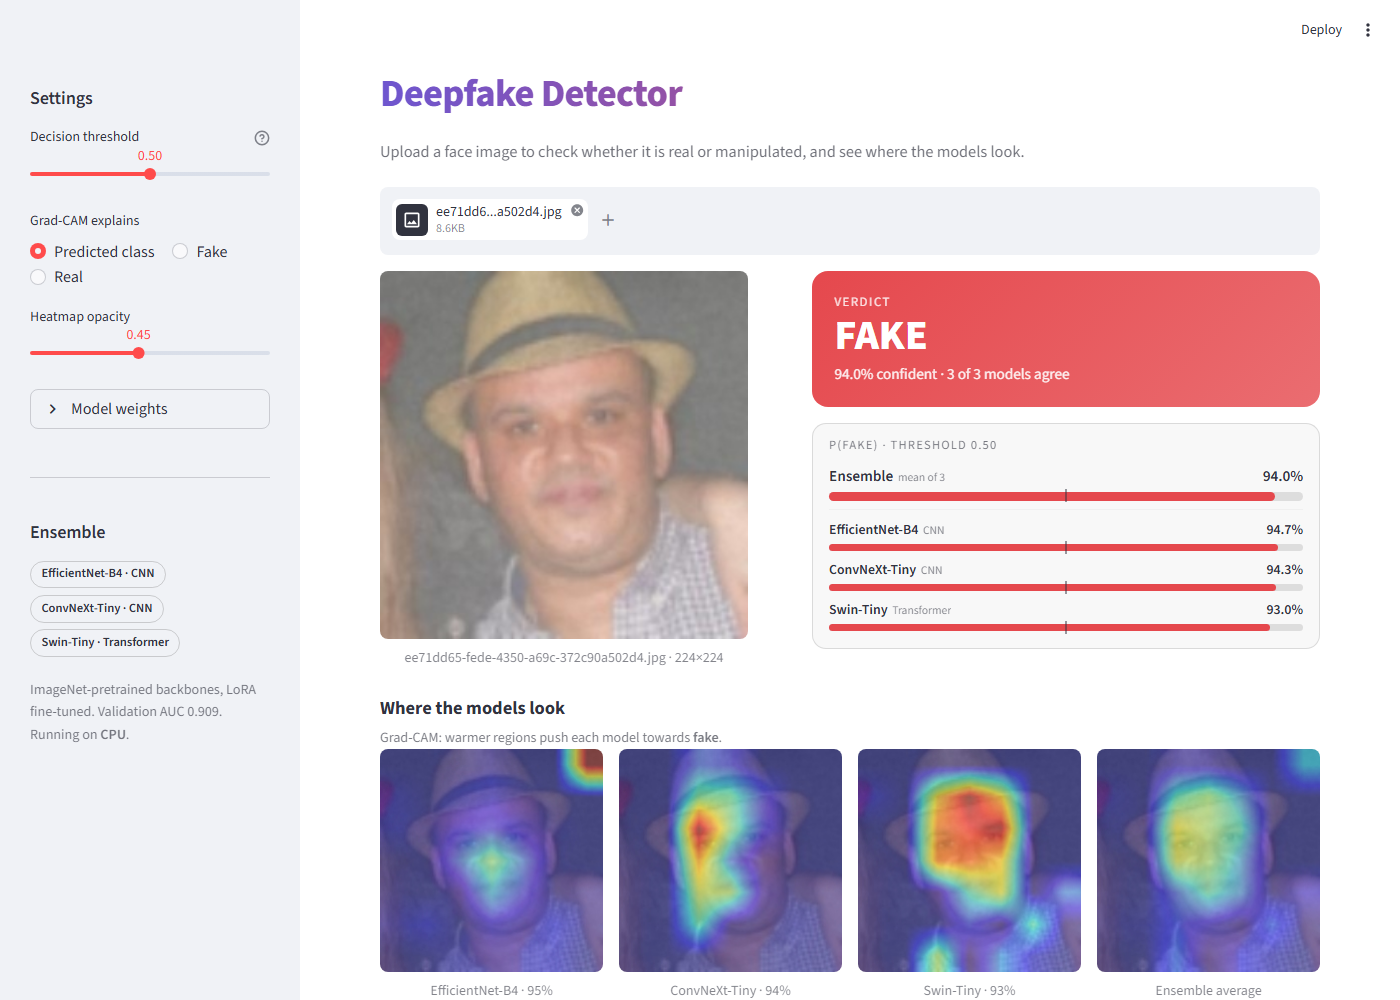
\includegraphics[width=0.85\linewidth]{streamlit_fake_prediction.png}
\caption{A fake training image: FAKE at 94\%, all three models agree. Grad-CAM (explaining \emph{fake}) concentrates on the face for ConvNeXt and Swin.}
\end{figure}

\begin{figure}[H]
\centering
\begin{subfigure}[t]{0.49\linewidth}\centering
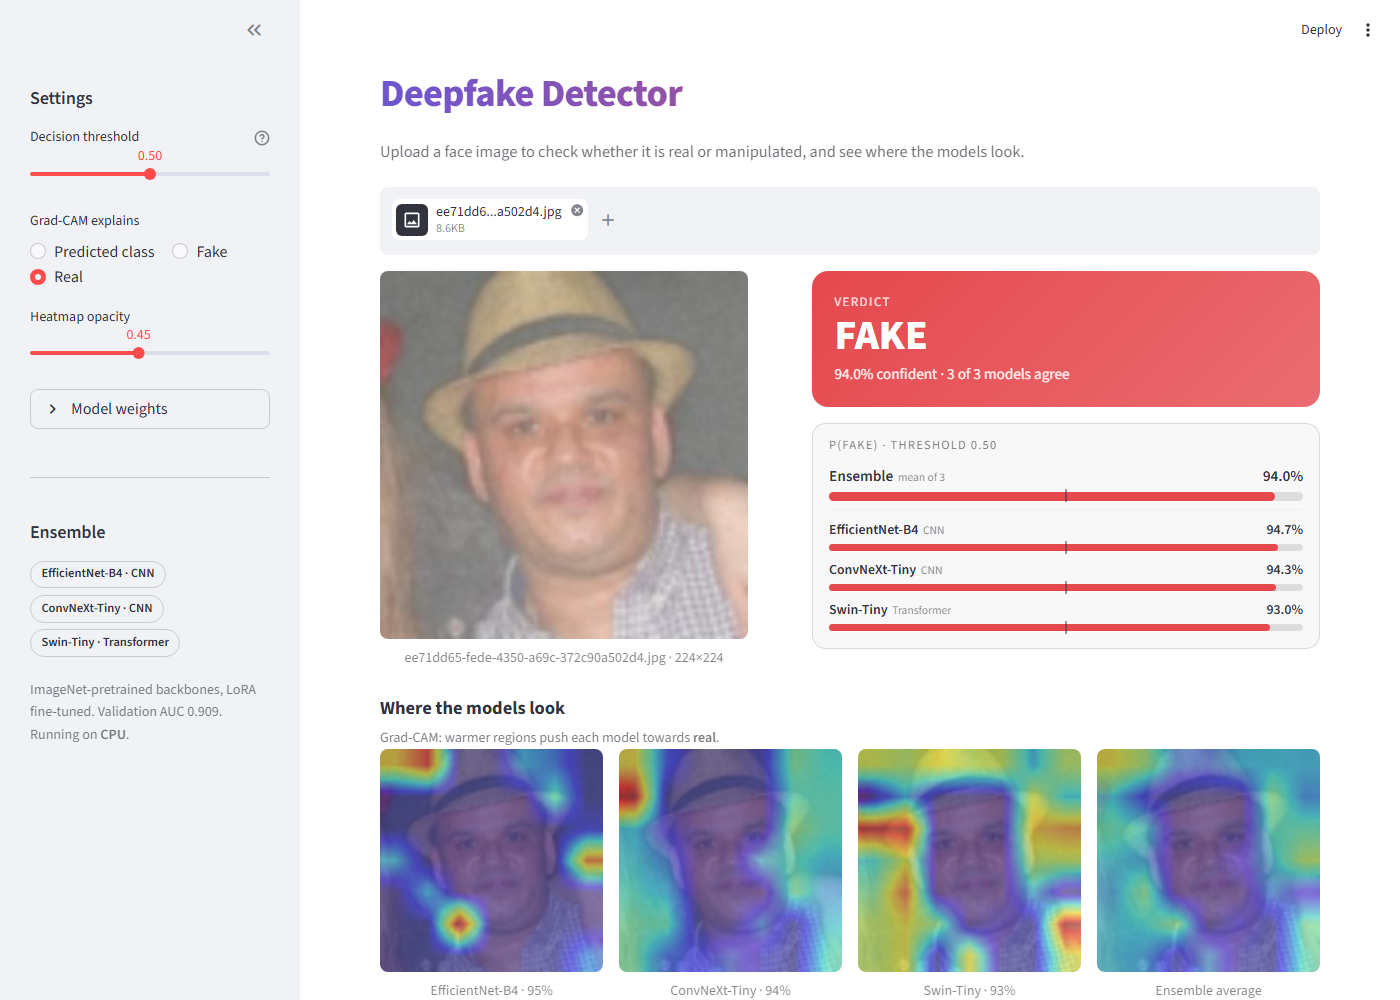
\includegraphics[width=\linewidth]{streamlit_fake_gradcam_real.png}
\caption{Same fake image, Grad-CAM set to \emph{Real}: the little evidence for ``real'' lies on background and edges, not the face.}
\end{subfigure}\hfill
\begin{subfigure}[t]{0.49\linewidth}\centering
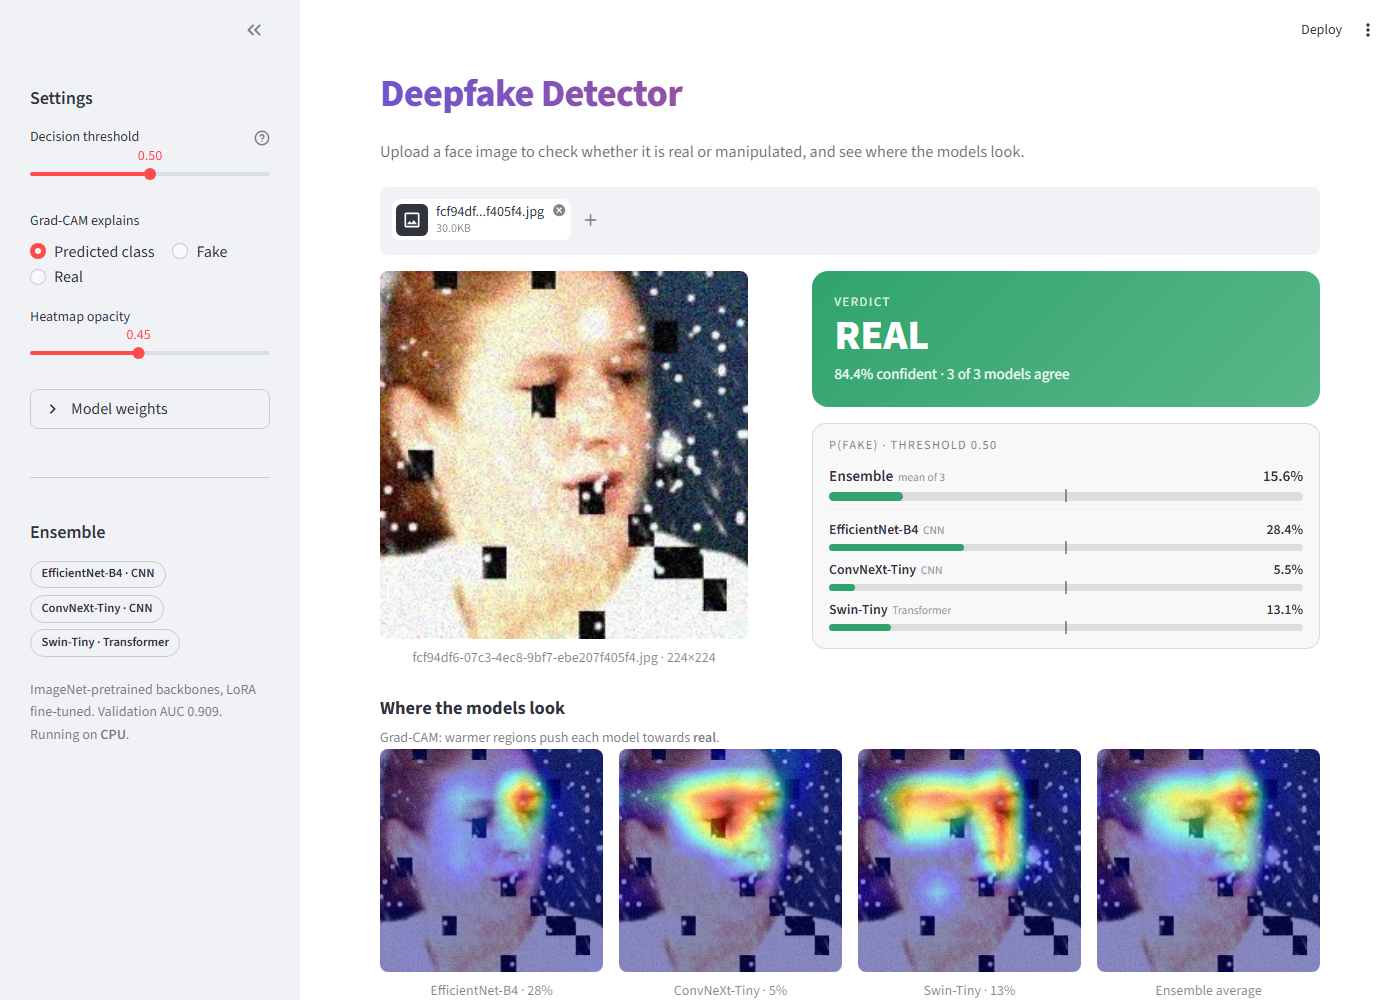
\includegraphics[width=\linewidth]{streamlit_real_prediction.png}
\caption{A heavily corrupted real image (noise, occlusion boxes): REAL at 84\%, all models agree.}
\end{subfigure}
\caption{Grad-CAM targets and a real example.}
\end{figure}

\subsection{Grad-CAM computation}
For each model we use its last feature stage (\texttt{backbone.features[-1]}, a $7\times7$ grid of $K$ channels $A^k$):
\begin{enumerate}
\item forward the image and take the fake logit $z$; choose the target score $s=+z$ (explain \emph{fake}) or $s=-z$ (explain \emph{real});
\item back-propagate $s$ and average the gradient over the grid: $\alpha_k = \frac{1}{49}\sum_{i,j}\partial s/\partial A^k_{ij}$;
\item $\mathrm{CAM} = \mathrm{ReLU}\big(\sum_k \alpha_k A^k\big)$, upsampled bilinearly to $224\times224$, min--max normalised and overlaid (Swin's channels-last map is permuted first). The ensemble map is the mean of the three normalised maps.
\end{enumerate}
\textbf{Settings.} \emph{Fake} ($s=+z$) highlights regions that raise the fake score --- where a model sees manipulation evidence. \emph{Real} ($s=-z$) highlights regions that lower it --- evidence for authenticity, i.e.\ counter-evidence on an image judged fake. \emph{Predicted class} (default) picks the sign of the ensemble verdict, so the map always explains the displayed decision. Grad-CAM shows where a model looked at $7\times7$ resolution; it is an aid to interpretation, not proof of manipulation.

% =====================================================================
\section{Challenges, Limitations and Conclusion}
\begin{itemize}
\item \textbf{Noisy labels.} About 8\% of labels appear flipped, capping validation AUC near 0.92 and making differences below $\approx$0.01 indistinguishable from noise on 1{,}400 images. We addressed it with label smoothing, a small trainable-parameter budget and checkpoint selection; we did not relabel data.
\item \textbf{Optimistic validation.} Repeated source photos across the random split inflate validation scores somewhat.
\item \textbf{Robustness untested on the hidden variants.} Augmentation covers the corruption families seen in the data but not, e.g., JPEG re-compression; we did not measure AUC under synthetic degradations.
\item \textbf{Limited tuning.} Auxiliary-loss weights and LoRA rank were not tuned by systematic search.
\end{itemize}
\noindent In summary, parameter-efficient LoRA fine-tuning of three diverse ImageNet backbones, combined with test-like augmentation and consistency/contrastive regularisation, gives a compact detector (1.0M/0.5M/0.6M trainable parameters) that reaches 0.909 validation AUC --- close to the $\approx$0.92 ceiling imposed by label noise --- and explains its decisions with per-model Grad-CAM.

\end{document}
